\section{Robustness and Falsification}
\label{sec:robustness}

\subsection{Triple horse race}
\label{subsec:robust_horserace}

Section~\ref{sec:results} reported the triple horse race (Table~\ref{tab:panel_three_pronged}, column~4), which estimates the three friction-PCI interactions jointly under pair and product--year fixed effects. We collect the implications here. The three coefficients retain their signs: $\hat{\gamma}_{\text{FATF}} = -0.076$, $\hat{\gamma}_{\text{AMLD}} = +0.129$ ($p = 0.050$), $\hat{\gamma}_{\text{FDI}} = -0.110$ ($p = 0.075$). Three points follow.

First, the AMLD coefficient is not absorbed by FATF or FDI exposure. Its magnitude in the horse race ($+0.129$) is statistically indistinguishable from its magnitude in the single-channel specification ($+0.141$). Regulatory harmonization captures a distinct channel from bank-side de-risking.

Second, the sign mirror across FATF and AMLD survives joint estimation. A confounder that produced opposite signs on opposite-direction friction shocks would have to vary jointly with the timing of FATF designations, the post-2017 EU period, and the FDI ratio of bilateral corridors. We know of no such variable.

Third, the FATF and FDI channels are partially substitutable in identification. The sum of the two negative coefficients ($-0.076 + -0.110 = -0.186$) is close to the single-channel magnitude of either, consistent with both indicators capturing slices of the same payment-friction increase.

\subsection{Kitchen sink and coverage attrition}
\label{subsec:robust_kitchen}

The kitchen-sink panel (Table~\ref{tab:panel_three_pronged}, column~5) adds $\text{diplo\_disagreement}_{ij,t} \times \text{PCI}_p$ and RTA controls. The sample halves from 2.82 million to 1.37 million observations because RTA and UN-voting coverage are incomplete. In this restricted sample $\hat{\gamma}_{\text{AMLD}}$ falls to $+0.023$ and $\hat{\gamma}_{\text{FDI}}$ falls to $-0.048$, both statistically indistinguishable from zero, while $\hat{\gamma}_{\text{FATF}}$ strengthens to $-0.290$ ($p = 0.098$).

We treat the attenuation as a power problem driven by coverage rather than a failure of the mechanism, for three reasons. First, the kitchen-sink yearly cross-sections (with the same RTA-restricted sample but only one shock at a time per year) preserve the AMLD coefficient at $+0.13$ to $+0.20$, significant at the 1\% level in every estimated year (2018--2020). The attenuation is a feature of the joint panel specification on the restricted sample, not of the AMLD shock per se. Second, the kitchen-sink yearly specification estimates $\text{diplo\_disagreement} \times \text{PCI}$ as positive ($+0.062$ to $+0.086$, significant at the 1\% level in every estimated year (2018--2020)). A negative effect would be expected if diplomatic distance were the omitted variable driving the complexity penalty; the positive sign rules this interpretation out. Third, EU membership in our sample is highly correlated with regulatory infrastructure that the RTA indicator and UN-voting distance capture only partially. The restricted sample is concentrated among advanced economies where both EU membership and AMLD compliance covary with omitted regulatory variables, which mechanically attenuates the AMLD coefficient. Columns~4 and~5 therefore bound the AMLD effect: column~4 (full sample, joint estimation) is the upper bound; column~5 (restricted sample, joint estimation with controls) is the lower bound.

\subsection{Single-channel specification curve}

Table~\ref{tab:robustness} summarizes robustness across 10 specification variants for the FDI-derisked $\times$ PCI interaction, each estimated year by year from 2018 to 2023. The baseline coefficient (mean $= -0.302$, significant in 6/6 years) is stable across alternative PCI measurement (Method of Reflections), exclusion of entrepot countries, exclusion of China, exclusion of commodities (HS chapters 01--27), pre-COVID and post-COVID subsamples, and alternative de-risking thresholds (25\% and 75\%). The sole exception is OLS on $\log(1 + \text{trade})$, which produces near-zero coefficients, consistent with the known bias of OLS in the presence of heteroskedasticity and zero trade flows \citep{SantosSilva2006_ppml}.

\begin{table}[htbp]
\centering
\caption{Robustness: Specification Summary}
\label{tab:robustness}
\begin{threeparttable}
\small
\begin{tabular}{lccc}
\toprule
Specification & Mean coef. & Mean SE & Sig. years \\
\midrule
Baseline & -0.302*** & (0.042) & 6/6 \\
Alt. PCI (Method of Reflections) & -0.290*** & (0.041) & 6/6 \\
Excl. entrepot countries & -0.303*** & (0.048) & 6/6 \\
Excl. China & -0.289*** & (0.041) & 6/6 \\
Excl. commodities (HS 01--27) & -0.308*** & (0.060) & 6/6 \\
Pre-COVID only (2018--2019) & -0.251*** & (0.042) & 2/2 \\
Post-COVID only (2021--2023) & -0.321*** & (0.039) & 3/3 \\
OLS log(1+trade) & 0.013*** & (0.005) & 4/6 \\
De-risking threshold: 25\% & -0.341*** & (0.056) & 6/6 \\
De-risking threshold: 75\% & -0.255*** & (0.039) & 6/6 \\
\bottomrule
\end{tabular}
\begin{tablenotes}
\tablenote{Each row reports the mean coefficient and pooled standard error across year-by-year PPML cross-sections (2018--2023). ``Sig. years'' counts years where $p < 0.05$. Baseline specification: $\text{Derisked} \times \text{PCI}$ with exporter, importer, and product FE. * $p < 0.10$, ** $p < 0.05$, *** $p < 0.01$.}
\end{tablenotes}
\end{threeparttable}
\end{table}

The temporal pattern is informative: pre-COVID coefficients ($-0.22$ to $-0.28$) are weaker than post-COVID ($-0.26$ to $-0.38$). Panel pair-FE estimates confirm this asymmetry: pre-COVID $\hat{\gamma} = -0.234$ ($p = 0.008$) versus post-COVID $\hat{\gamma} = -0.493$ ($p < 0.001$). The complexity penalty from FDI de-risking accelerates over time. Section~\ref{subsec:robust_speccurve} below visualizes the panel analogue of this curve in a single forest plot.

\subsection{Panel specification curve}
\label{subsec:robust_speccurve}

The yearly cross-sections in Section~\ref{subsec:robust_horserace} test stability across years and PCI measurement choices. We complement them with a panel specification curve that perturbs the four-fixed-effect baseline along ten dimensions: lag structure of the de-risking indicator, choice of friction proxy, country and product subsamples, sample period, fixed-effect structure, and estimator. (We index the specifications R0, R1, R2, R3, R5--R10; the gap at R4 reflects an alternative PCI measurement check that requires a Method-of-Reflections PCI not computed in this paper and is left for future work.) The dependent variable and the interaction of interest, $\text{Derisked}_{ij,t} \times \text{PCI}_{p,t}$, are held fixed; one feature changes per row. Table~\ref{tab:robustness_speccurve} reports the results, and Figure~\ref{fig:spec_curve_panel} plots them.

\begin{table}[htbp]
\centering
\caption{Robustness: Panel Specification Curve}
\label{tab:robustness_speccurve}
\begin{threeparttable}
\footnotesize
\setlength{\tabcolsep}{4pt}
\begin{tabular}{llccccc}
\toprule
ID & Specification & Coefficient & Std. Error & 95\% CI Low & 95\% CI High & N \\
\midrule
R0 & Baseline & -0.3084$^{***}$ & (0.0994) & -0.5032 & -0.1137 & 1,689,462 \\
R1 & Lag-1 derisked & -0.2706$^{***}$ & (0.0987) & -0.4641 & -0.0771 & 1,689,462 \\
R2 & Lag-2 derisked & -0.2677$^{***}$ & (0.0965) & -0.4568 & -0.0785 & 1,689,462 \\
R3 & RPW friction only & 0.0895$^{**}$ & (0.0409) & 0.0093 & 0.1696 & 22,842 \\
R5 & Excl. entrepots & -0.3414$^{***}$ & (0.1133) & -0.5635 & -0.1193 & 1,507,948 \\
R6 & Excl. China & -0.1604$^{**}$ & (0.0657) & -0.2891 & -0.0317 & 1,662,954 \\
R7 & Excl. commodities (HS01-27) & -0.2692$^{***}$ & (0.1021) & -0.4693 & -0.0691 & 1,195,615 \\
R8 & Pre-COVID (year $\leq$ 2019) & -0.1807$^{*}$ & (0.1070) & -0.3903 & 0.0289 & 550,652 \\
R9 & No pair FEs & -0.3084$^{***}$ & (0.0476) & -0.4017 & -0.2151 & 1,691,154 \\
R10 & OLS log(1+trade) & -0.0066 & (0.0137) & -0.0334 & 0.0202 & 1,692,000 \\
\bottomrule
\end{tabular}
\begin{tablenotes}
\tablenote{Each row is a separate PPML estimation of $\text{Derisked}_{ij,t} \times \text{PCI}_{p,t}$ with exporter--year, importer--year, pair, and HS2 fixed effects (the four-FE baseline R0). R1 and R2 replace contemporaneous de-risking with one- and two-year lags. R3 substitutes the retail remittance-price-weighted (RPW) friction index for the de-risking indicator. R5 drops the four standard entrep\^ot economies (Hong Kong, Singapore, Netherlands, Belgium). R6 drops China. R7 drops HS chapters 01--27 (commodities). R8 restricts to pre-COVID years ($\leq 2019$). R9 drops pair fixed effects. R10 estimates OLS on $\ln(1+\text{trade})$. Standard errors clustered at the country-pair level in parentheses. * $p < 0.10$, ** $p < 0.05$, *** $p < 0.01$.}
\end{tablenotes}
\end{threeparttable}
\end{table}

\begin{figure}[htbp]
\centering
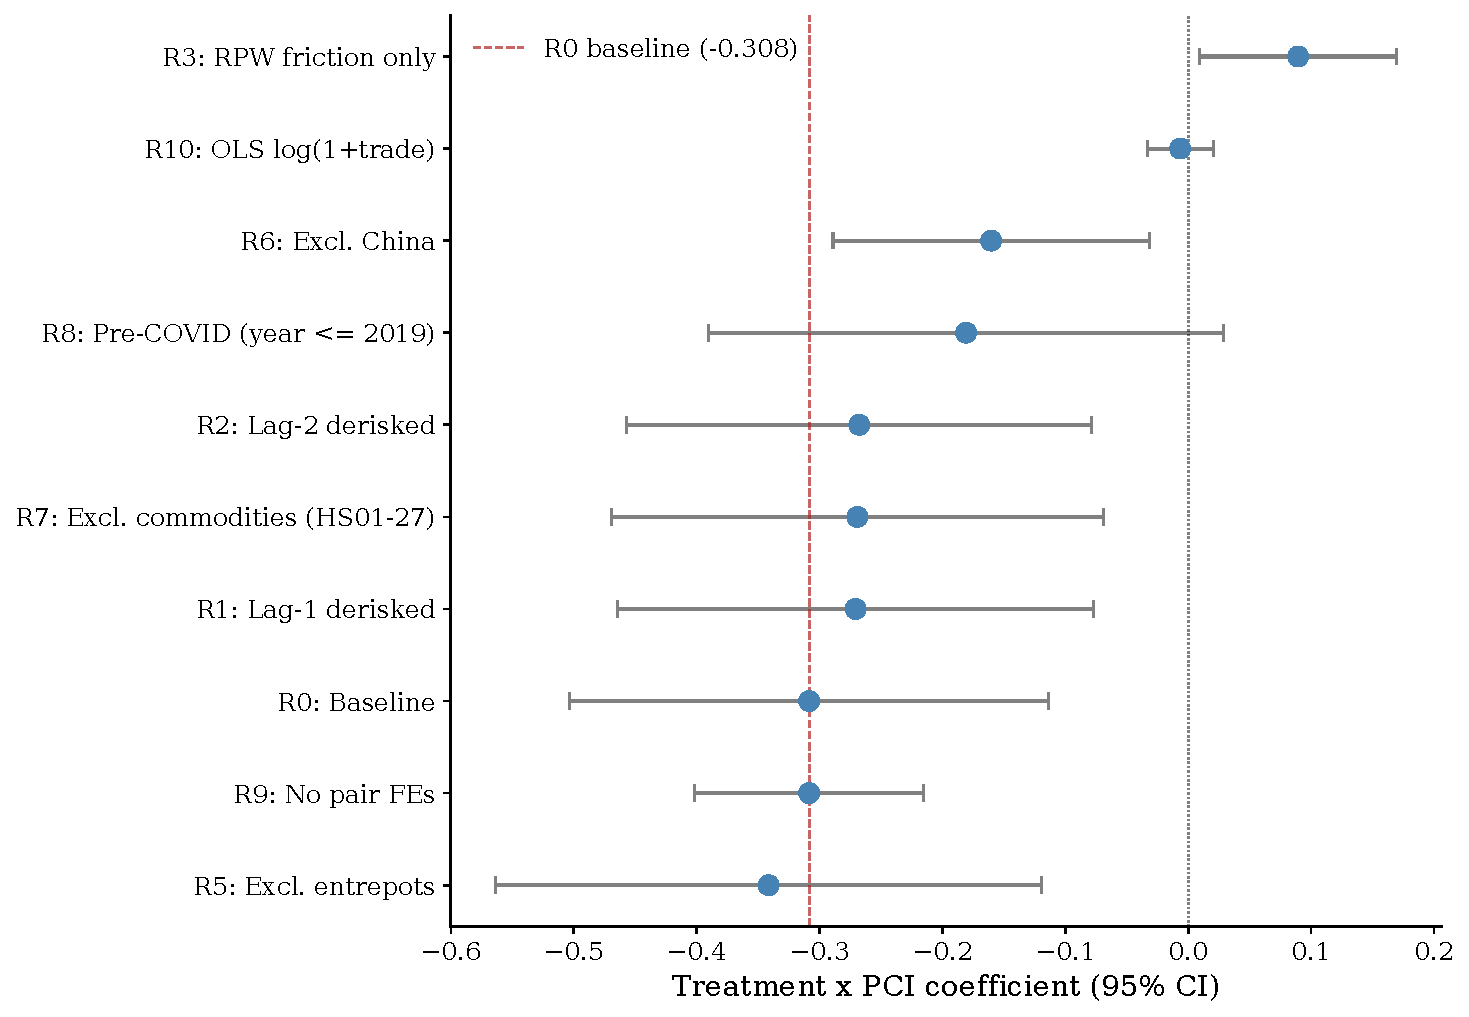
\includegraphics[width=0.8\textwidth]{figures/11_robustness/specification_curve.pdf}
\caption{Panel Specification Curve: $\text{Derisked} \times \text{PCI}$ Across Ten Variants}
\label{fig:spec_curve_panel}
\begin{minipage}{0.9\textwidth}
\footnotesize \textit{Notes.} Coefficient estimates and 95\% confidence intervals across the ten specification variants in Table~\ref{tab:robustness_speccurve}. The dashed vertical line marks zero. R0 is the four-fixed-effect PPML baseline.
\end{minipage}
\end{figure}

The headline pattern is preserved across nine of the ten specifications. The de-risking--complexity interaction stays negative and statistically distinguishable from zero at the 5\% level in seven specifications (R0, R1, R2, R5, R6, R7, R9), at the 10\% level in R8 (pre-COVID), and flips sign only in R3 (RPW) and goes to near-zero in R10 (OLS). Magnitudes range from $-0.160$ (R6, excluding China) to $-0.341$ (R5, excluding entrep\^ots).

Three points warrant explicit discussion.

First, the R0 baseline coefficient of $-0.308$ differs from the $\hat{\gamma}_{\text{FDI}} = -0.135$ reported in Section~\ref{subsec:fdi} and from the $-0.198$ headline in the falsification panel (Section~\ref{subsec:falsification_placebo}, F0). The three numbers come from different specifications. The Section~\ref{subsec:fdi} estimate uses pair plus product--year fixed effects on the full panel; the falsification F0 estimate adds exporter--year, importer--year, pair, and HS2 fixed effects on a stratified 3{,}000-pair subsample with the $\ln(\text{dist})$ filter applied; the R0 estimate uses the same four-FE structure as F0 but on the full panel without the $\ln(\text{dist})$ filter, so its identifying sample is larger. The estimates are coefficients from related but not identical models; they should not be expected to coincide. The qualitative finding---negative sign, statistical separation from zero, magnitudes in the $-0.13$ to $-0.34$ band---is the cross-specification statement.

Second, R6 (excluding China) halves the magnitude to $-0.160$. China contributes a meaningful share of the headline magnitude, both because of its volume and because of its position as a high-complexity exporter into corridors with varying de-risking exposure. We treat this as a sensitivity result rather than a refutation: the sign and significance survive the exclusion, and a coefficient of $-0.160$ on a one-standard-deviation shift in PCI still corresponds to a $14.8\%$ trade-flow reduction. The result speaks to where the average effect comes from, not to whether the effect exists.

Third, R3 (RPW friction only) flips sign to $+0.090$ ($p = 0.029$) on a much smaller sample (22{,}842 observations). The RPW index measures retail remittance prices, a different friction channel from correspondent-banking de-risking. Retail remittance corridors and complex-goods trade corridors do not coincide cleanly; the RPW data covers a small set of country pairs heavily weighted toward labor-sending corridors. We do not interpret the R3 coefficient as evidence against the de-risking--complexity channel; it is evidence about a different channel measured on a different sample. R10 (OLS on $\ln(1+\text{trade})$) collapses to $-0.007$, the well-known PPML--OLS gap on count and positive-with-mass-at-zero data \citep{SantosSilva2006_ppml}; the panel specification curve in our setting confirms the same pattern that the yearly curve already showed.

The bottom line of the panel specification curve: the negative interaction survives lag perturbation, entrep\^ot exclusion, China exclusion, commodity exclusion, the pre-COVID subsample, and the four-FE-without-pair structure; the OLS--PPML gap and a non-comparable friction proxy account for the two outliers.

\subsection{Lag and lead tests}
\label{subsec:lags_leads}

Three layers of evidence speak to the endogeneity of contemporaneous de-risking: the lagged-friction tests reported here, the de-risking reduced form already in Section~\ref{sec:results}, and a forward-looking placebo using a one-year lead. If the contemporaneous correlation reflects a payment-friction shock that causes complex trade to decline, lagged de-risking should still predict differential reductions in complex trade; a lead specification, by contrast, should be null under standard pre-trends logic. We estimate both on the 3{,}000-pair subsample and the four-FE PPML structure used in the falsification panel of Section~\ref{subsec:falsification_placebo}, so the contemporaneous benchmark is the F0 estimate ($-0.198$).

\begin{table}[htbp]
\centering
\caption{Endogeneity: Lag and Lead Specifications}
\label{tab:endogeneity_panel}
\begin{threeparttable}
\small
\begin{tabular}{lccc}
\toprule
 & (1) & (2) & (3) \\
 & Lag-1 & Lag-2 & Lead-1 \\
\midrule
Treatment $\times$ PCI & -0.2773$^{***}$ & -0.2744$^{***}$ & -0.3546$^{***}$ \\
 & (0.1001) & (0.0978) & (0.1020) \\
Treatment & -0.0889$^{*}$ & -0.0455 & -0.1340$^{**}$ \\
 & (0.0520) & (0.0491) & (0.0606) \\
\midrule
Observations & 1,496,762 & 1,479,372 & 1,239,202 \\
Exporter-year FE & Yes & Yes & Yes \\
Importer-year FE & Yes & Yes & Yes \\
Pair FE & Yes & Yes & Yes \\
Product (HS2) FE & Yes & Yes & Yes \\
\bottomrule
\end{tabular}
\begin{tablenotes}
\tablenote{PPML estimation on the 3{,}000-pair subsample (2{,}000 FDI-derisked treated pairs plus 1{,}000 control pairs), 2018--2023, using the same sample filter as the falsification panel of Table~\ref{tab:falsification_panel}. Column (1) replaces $\text{Derisked}_{ij,t}$ with $\text{Derisked}_{ij,t-1}$; column (2) with $\text{Derisked}_{ij,t-2}$; column (3) with $\text{Derisked}_{ij,t+1}$. Dependent variable: bilateral trade value at the country-pair--HS2--year level. All specifications include exporter--year, importer--year, pair, and HS2 fixed effects. Standard errors clustered at the country-pair level in parentheses. * $p < 0.10$, ** $p < 0.05$, *** $p < 0.01$.}
\end{tablenotes}
\end{threeparttable}
\end{table}

The lag results provide positive evidence for the channel. The one-year lag, $\text{Derisked}_{ij,t-1}$, yields an interaction coefficient of $-0.277$ ($p = 0.006$), and the two-year lag, $\text{Derisked}_{ij,t-2}$, yields $-0.274$ ($p = 0.005$). Both magnitudes are within sampling variation of the contemporaneous F0 benchmark of $-0.198$, and both are significant at the 1\% level. Lagged de-risking continues to predict differential complex-trade reductions, consistent with a causal payment-friction channel that propagates over multi-year horizons.

The lead test is more difficult to interpret. Substituting $\text{Derisked}_{ij,t+1}$ produces an interaction coefficient of $-0.355$ ($p = 0.0005$), more negative than the contemporaneous estimate. Two interpretations are available. The first is anticipation or pre-trends: complex trade in soon-to-be-derisked corridors may already have been declining before the FDI ratio crossed the de-risking threshold. The second, which we view as more plausible given the construction of the de-risking indicator, is mechanical persistence. A corridor's derisked status is near-permanent in our sample, so $\text{Derisked}_{ij,t+1}$ is highly correlated with $\text{Derisked}_{ij,t}$ within the same pair. Under this interpretation the lead test is not a true placebo but a noisier re-estimation of the contemporaneous effect on a sample shifted forward by one year. We cannot fully separate the two interpretations without an event-time design that exploits the timing of the FDI ratio crossing the 50\% threshold. We leave a sharper event-study to future work and note that the lag tests, which use earlier values of the same persistent indicator and so do not face the same forward-correlation concern, do support the causal interpretation.

On balance, the lag tests support the causal interpretation of the headline; the lead test is inconclusive due to corridor-level persistence in de-risking status.

\subsection{Falsification: placebo gravity-PCI interactions}
\label{subsec:falsification_placebo}

We probe the specificity of the friction--complexity channel by substituting standard gravity variables for the FDI-derisking shock in the PCI interaction. If the headline complexity penalty reflects a genuine payment-infrastructure mechanism, the headline coefficient should survive the addition of these placebo interactions, and the placebo coefficients themselves should be small for variables that are pure trade-cost shifters.

We estimate six PPML specifications on a 3{,}000-pair subsample (2{,}000 treated and 1{,}000 control pairs, 2018--2023, $1{,}684{,}198$ observations). Each specification includes pair, exporter--year, importer--year, and HS2 fixed effects. Specification F0 reports the headline $\text{Derisked} \times \text{PCI}$ alone. Specifications F1--F5 add a placebo gravity--PCI interaction (log distance, common language, contiguity, common colony, RTA coverage) one at a time. Table~\ref{tab:falsification_panel} reports the results.

\begin{table}[htbp]
\centering
\caption{Falsification: Placebo Gravity--PCI Interactions}
\label{tab:falsification_panel}
\begin{threeparttable}
\scriptsize
\setlength{\tabcolsep}{4pt}
\begin{tabular}{lcccccc}
\toprule
 & (1) & (2) & (3) & (4) & (5) & (6) \\
 & Baseline & + Distance & + Language & + Contiguity & + Colony & + RTA \\
\midrule
Derisked $\times$ PCI & -0.1976$^{***}$ & -0.2000$^{***}$ & -0.2049$^{***}$ & -0.1991$^{***}$ & -0.2013$^{***}$ & -0.1863$^{***}$ \\
 & (0.0607) & (0.0565) & (0.0597) & (0.0606) & (0.0610) & (0.0633) \\
\midrule
$\ln(\text{dist}) \times \text{PCI}$ & -- & 0.0061 & -- & -- & -- & -- \\
 & -- & (0.0438) & -- & -- & -- & -- \\
Common language $\times$ PCI & -- & -- & -0.0800 & -- & -- & -- \\
 & -- & -- & (0.1590) & -- & -- & -- \\
Contiguity $\times$ PCI & -- & -- & -- & -0.1486$^{**}$ & -- & -- \\
 & -- & -- & -- & (0.0587) & -- & -- \\
Colony $\times$ PCI & -- & -- & -- & -- & -0.2128$^{***}$ & -- \\
 & -- & -- & -- & -- & (0.0782) & -- \\
RTA $\times$ PCI & -- & -- & -- & -- & -- & 0.0575 \\
 & -- & -- & -- & -- & -- & (0.0483) \\
\midrule
Observations & 1,684,198 & 1,684,198 & 1,649,700 & 1,684,198 & 1,649,700 & 1,684,198 \\
Pair $\times$ year FE & Yes & Yes & Yes & Yes & Yes & Yes \\
Exporter-year, Importer-year FE & Yes & Yes & Yes & Yes & Yes & Yes \\
Product (HS4) FE & Yes & Yes & Yes & Yes & Yes & Yes \\
\bottomrule
\end{tabular}
\begin{tablenotes}
\tablenote{PPML estimation on a 3{,}000-pair subsample (2{,}000 FDI-derisked treated pairs plus 1{,}000 control pairs), 2018--2023. Dependent variable: bilateral trade value at the country-pair--HS2--year level. All specifications include pair, exporter--year, importer--year, and HS2 fixed effects. Each placebo interaction enters one column at a time alongside the headline $\text{Derisked} \times \text{PCI}$ term. Standard errors clustered at the country-pair level in parentheses. * $p < 0.10$, ** $p < 0.05$, *** $p < 0.01$.}
\end{tablenotes}
\end{threeparttable}
\end{table}

The headline coefficient is fully robust. $\hat{\gamma}_{\text{FDI}}$ ranges from $-0.186$ (F5, RTA $\times$ PCI) to $-0.205$ (F2, common language $\times$ PCI), and is significant at the 1\% level in every specification. The complexity penalty from FDI de-risking is not absorbed by any standard gravity--PCI interaction.

The placebo coefficients split. Three of five placebos are null. $\ln(\text{dist}) \times \text{PCI}$ enters at $+0.006$ ($p = 0.890$), $\text{comlang} \times \text{PCI}$ at $-0.080$ ($p = 0.615$), and $\text{rta} \times \text{PCI}$ at $+0.058$ ($p = 0.234$). Geographic distance, shared official language, and RTA coverage do not differentially penalize complex products in the de-risked-pair sample. These three placebos are pure trade-cost shifters, and their null loadings on the complexity interaction are the cleanest negative result the test produces.

The remaining two placebos load. Contiguity $\times$ PCI enters at $-0.149$ ($p = 0.011$) and common-colony $\times$ PCI at $-0.213$ ($p = 0.007$). Both significant at the 5\% or 1\% level. We interpret this as a partial falsification, not a clean win.

The interpretation that follows: contiguity and colonial ties are not pure trade-cost shifters. Contiguous neighbors share correspondent-banking infrastructure, currency arrangements, and cross-border payment systems that bundle with geography. Former-colony pairs typically inherit linked banking systems, common legal frameworks, and currency pegs that persist long after independence. The complexity penalty observed in those interactions is consistent with shared payment-system structure rather than an unrelated channel: contiguous and post-colonial pairs are precisely the pairs where the underlying payment architecture is most likely to be co-determined with the FDI relationship. The 3/5 clean nulls (distance, language, RTA) and the institutional-tie loadings on contiguity and colony are jointly consistent with the payment-friction story; they are inconsistent with a pure-trade-cost story, in which the distance interaction should also have loaded.

The headline channel passes the three sharpest placebo tests and shows expected loadings on the two institutional-tie placebos, while $\hat{\gamma}_{\text{FDI}}$ remains in the $-0.186$ to $-0.205$ band across all six specifications.

\subsection{Confounder check: complex exporters and friction exposure}
\label{subsec:falsification_confounder}

A direct confounder for the complexity penalty is a country-level correlation between export complexity and exposure to friction shocks: complex exporters might be more likely to be greylisted or de-risked for reasons unrelated to the payment channel. Figure~\ref{fig:pci_treatment} plots country-level mean PCI of exports against FATF exposure (years on the greylist between 2018 and 2023).

\begin{figure}[htbp]
\centering
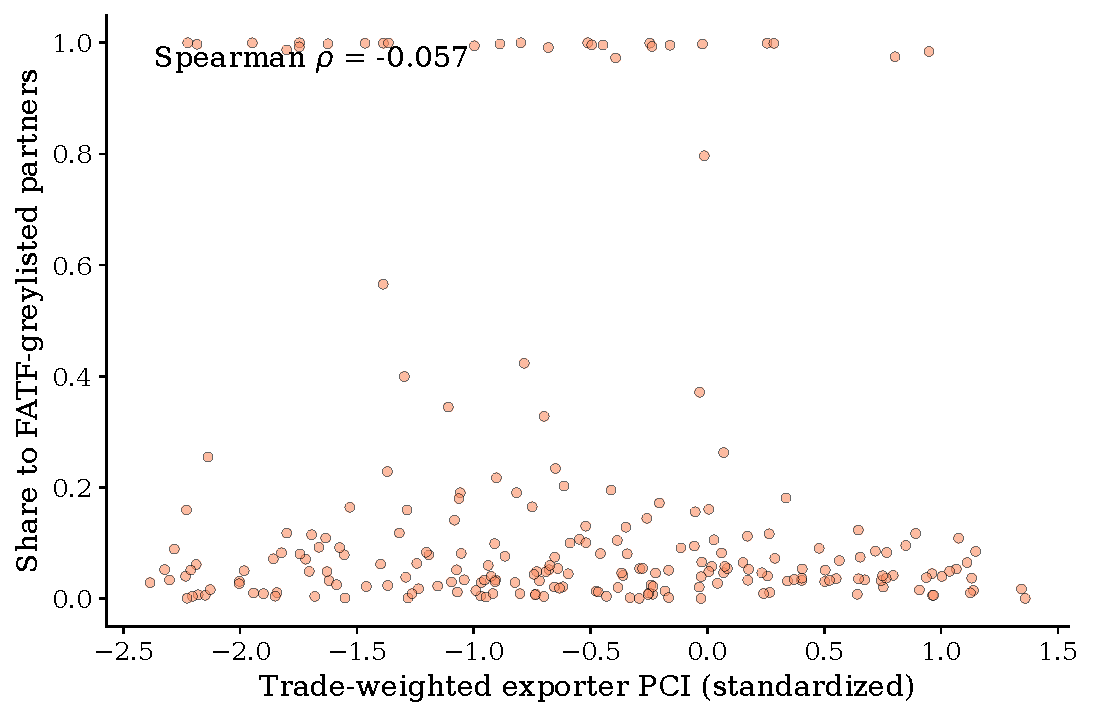
\includegraphics[width=0.8\textwidth]{figures/13_figures/fig_pci_treatment_correlation.pdf}
\caption{Country PCI of Exports vs.\ FATF Greylist Exposure}
\label{fig:pci_treatment}
\begin{minipage}{0.9\textwidth}
\footnotesize \textit{Notes.} Each point is a country. Horizontal axis: country-level mean PCI of exports over 2018--2023. Vertical axis: years on the FATF greylist between 2018 and 2023. The flat slope rules out the interpretation that complex exporters get greylisted more.
\end{minipage}
\end{figure}

The cross-country relationship is flat. Greylisted countries are spread across the export-complexity distribution rather than concentrated at the high-complexity end. The complexity penalty estimated in Section~\ref{sec:results} therefore does not arise from complex exporters being differentially greylisted.

\subsection{Auxiliary falsification tests}

We also conduct three auxiliary falsification tests on the full panel sample.

\paragraph{Friction $\times$ Perishability.} Replacing PCI with a perishability indicator tests whether the friction shocks affect perishable goods differently. In cross-sections, the interaction is positive and significant in 4/6 years. In the panel with pair fixed effects, the coefficient is $0.149$ ($p = 0.394$), which is null. The cross-sectional result captures between-corridor differences in perishable-goods geography rather than a causal friction channel.

\paragraph{Commodity-only subsample.} Restricting the sample to HS chapters 01--27 (primary commodities) produces a null interaction in the panel ($-0.082$, $p = 0.433$). The complexity penalty is driven by manufactured and complex goods, not raw commodities.

\subsection{AMLD diversion check}

A residual interpretation of the AMLD coefficient is that complex trade rerouted into EU corridors as non-EU corridors got greylisted. The triple horse race already controls directly for FATF exposure, and the AMLD coefficient is preserved. In addition, the AMLD coefficient is positive and significant in 2018 (a year in which the only major FATF designation was Pakistan), and the magnitude is comparable in 2018 and 2023, despite very different greylisting compositions across the two years. A diversion-only story implies that the AMLD coefficient should track the size of the greylisted footprint; the data do not show such a pattern.

\subsection{Permutation test}

We conduct a permutation test on the panel subsample, randomly reassigning FDI-derisked status across country pairs 50 times and re-estimating the $\text{Derisked} \times \text{PCI}$ coefficient. The null distribution has mean $-0.022$ and standard deviation $0.139$. Our baseline estimate of $-0.234$ lies in the left tail; the permutation $p$-value of $0.167$ does not reach conventional significance, a consequence of the limited number of successful convergences (12/50 permutations). The low convergence rate is itself informative: random de-risking assignments produce separation problems that the true de-risking pattern does not, indicating that real de-risking has a structured relationship with trade flows that random assignment lacks.
